\documentclass[a4paper,11pt]{article}
\usepackage[portuguese]{babel}
\usepackage{graphicx}
\usepackage{amsmath}
\usepackage{minted}
\usepackage{mdframed}


\usepackage[twoside,verbose,body={16cm,24cm},
left=25mm,top=20mm]{geometry}


\title{Cálculo de Programas \\ Resolução - Ficha 04}
\author{Eduardo Freitas Fernandes}
\date{2025}

\setminted{
	frame=single,
	tabsize=4,
	breaklines=true
}


\begin{document}
	
	\maketitle
	
	\noindent \underline{\textbf{Exercício 1}}\\
	\[
	\begin{aligned}
		&[\underline{k}, \underline{k}] = \underline{k} \\
		\equiv \  &\{\text{Universal-+}\}\\
		&\begin{cases}
			\underline{k} = \underline{k} \cdot i_1 \\
			\underline{k} = \underline{k} \cdot i_2
		\end{cases}\\
		\equiv \  &\{\text{Fusão-+}\}\\
		&\begin{cases}
			\underline{k} = \underline{k} \\
			\underline{k} = \underline{k}
		\end{cases}
	\end{aligned}
	\]
	
	\noindent \underline{\textbf{Exercício 2}}\\
	\[
	\begin{aligned}
		&fac \cdot [\underline{0}, succ] = [\underline{1}, mul \cdot \langle succ, fac \rangle ] \\
		\equiv \  &\{\text{Universal-+}\}\\
		&\begin{cases}
			fac \cdot [\underline{0}, succ] \cdot i_1 = \underline{1} \\
			fac \cdot [\underline{0}, succ] \cdot i_2 = mul \cdot \langle succ, fac \rangle
		\end{cases}\\
		\equiv \  &\{\text{Cancelamento-+}\}\\
		&\begin{cases}
			fac \cdot \underline{0} = \underline{1} \\
			fac \cdot succ = mul \cdot \langle succ, fac \rangle
		\end{cases}\\
		\equiv \  &\{\text{Absorção-+, point wise}\}\\
		&\begin{cases}
			\underline{fac \ 0} \ x = \underline{1} \ x \\
			(fac \cdot succ) \ n = (mul \cdot \langle succ, fac \rangle) \ n
		\end{cases}\\
		\equiv \  &\{\text{def. const, def. split, def. composição}\}\\
		&\begin{cases}
			fac \ 0 = 1 \\
			fac \ (succ \ n) = mul \ (succ \ n, fac \ n)
		\end{cases}\\
		\equiv \  &\{\text{def. succ, def. mul}\}\\
		&\begin{cases}
			fac \ 0 = 1 \\
			fac \ (n + 1) = (n + 1) * fac \ n
		\end{cases}\\
	\end{aligned}
	\]
	
	\newpage
	
	\noindent \underline{\textbf{Exercício 3}}\\
	\[
	\begin{aligned}
		&out \cdot in = id \\
		\equiv \  &\{\text{def. in, Fusão-+, Universal-+}\}\\
		&\begin{cases}
			out \cdot \underline{0} = id \cdot i_1 \\
			fac \cdot succ = id \cdot i_2
		\end{cases}\\
		\equiv \  &\{\text{Natural id, Absorção const, def. const}\}\\
		&\begin{cases}
			out \ 0 = i_1 \\
			out \cdot succ = i_2
		\end{cases}\\
		\equiv \  &\{\text{point wise, def. composição, def. succ}\}\\
		&\begin{cases}
			out \ 0 = i_1 \ () \\
			out \ (n + 1) = i_2 \ n
		\end{cases}
	\end{aligned}
	\]
	
	\noindent \underline{\textbf{Exercício 4}}
\begin{verbatim}
ghci> succ n = n+1
ghci> mul (a,b) = a*b
ghci> :{
ghci| out 0 = i1 ()
ghci| out n = i2 (n-1)
ghci| :}
ghci> fac = either (const 1) mul . (id -|- (split succ fac)) . out
ghci> fac 4
24
ghci> fac 6
720
\end{verbatim}
	
	\noindent \underline{\textbf{Exercício 5}}
	\begin{figure}[H]
		\centering
		\fbox{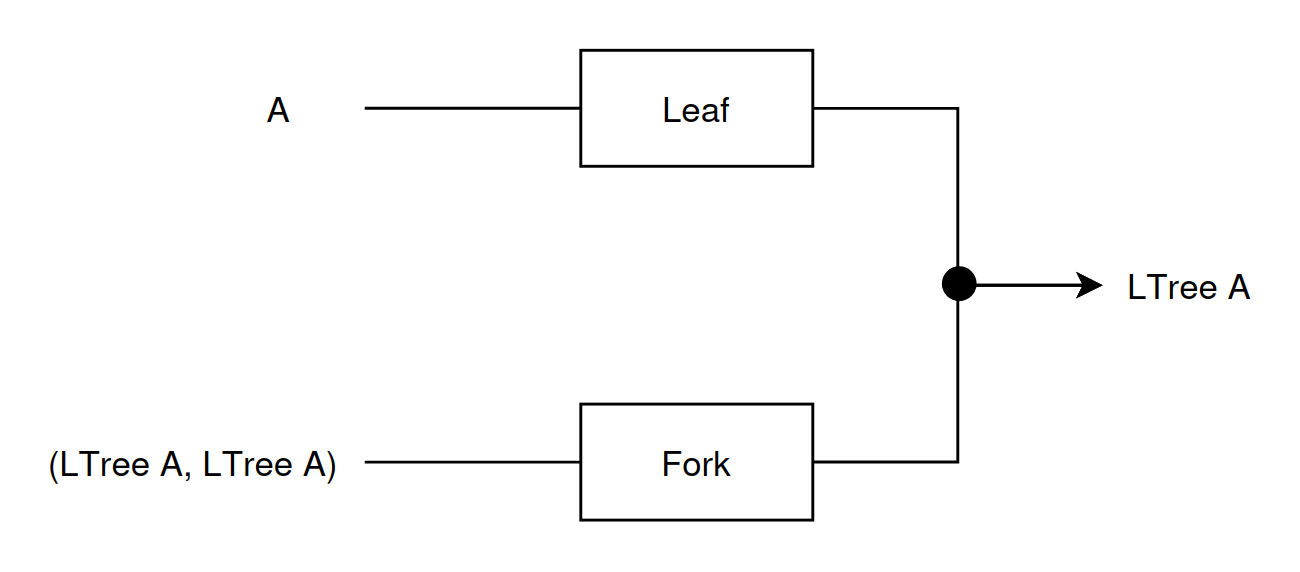
\includegraphics[width=0.6\textwidth]{ficha-04-5.png}}
	\end{figure}
	\[
	\begin{aligned}
		&out \cdot in = id \\
		\equiv \  &\{\text{def. in, Fusão-+, Universal-+}\}\\
		&\begin{cases}
			out \cdot Leaf = id \cdot i_1 \\
			out \cdot Fork = id \cdot i_2
		\end{cases}\\
		\equiv \  &\{\text{Natural id, point wise, def. composição}\}\\
		&\begin{cases}
			out \ (Leaf \ a) = i_1 \ a \\
			out \ (Fork \ (x, y)) = i_1 \ (x, y)
		\end{cases}
	\end{aligned}
	\]
	
	\noindent \underline{\textbf{Exercício 6}}\\
	\[
	\begin{aligned}
		&coassocl \cdot [id + i_1, i_2 \cdot i_2] = id \\
		\equiv \  &\{\text{Fusão-+, Universal-+}\}\\
		&\begin{cases}
			coassocl \cdot (id + i_1) = i_1 \\
			coassocl \cdot i_2 \cdot i_2 = i_2
		\end{cases}\\
		\equiv \  &\{\text{def-+, Fusão-+, Universal-+}\}\\
		&\begin{cases}
			\begin{cases}
				coassocl \cdot i_1 = i_1 \cdot i_1 \\
				coassocl \cdot i_2 \cdot i_1 = i_1 \cdot i_2
			\end{cases} \\
			coassocl \cdot i_2 \cdot i_2 = i_2
		\end{cases}\\
		\equiv \  &\{\text{?????}\}\\
		&\begin{cases}
			coassocl \cdot i_1 = i_1 \cdot i_1 \\
			\begin{cases}
				coassocl \cdot i_2 \cdot i_1 = i_1 \cdot i_2 \\
				coassocl \cdot i_2 \cdot i_2 = i_2
			\end{cases} \\
		\end{cases}\\
		\equiv \  &\{\text{Universal-+}\}\\
		&\begin{cases}
			coassocl \cdot i_1 = i_1 \cdot i_1 \\
			coassocl \cdot i_2 = [i_1 \cdot i_2, i_2]
		\end{cases}\\
		\equiv \  &\{\text{Universal-+}\}\\
		&coassocl = [i_1 \cdot i_1, [i_1 \cdot i_2, i_2]]
	\end{aligned}
	\]
	
	\noindent \underline{\textbf{Exercício 7}}
\begin{verbatim}
ghci> undistr (i1 ("CP", True))
("CP",Left True)
ghci> undistr (i2 ("LEI", 1))
("LEI",Right 1)	
ghci> (distr . undistr) (i2 ("LEI", 1))
Right ("LEI",1)
ghci> (distr . undistr) (i1 ("LEI", 1))
Left ("LEI",1)
\end{verbatim}
	
	\noindent \underline{\textbf{Exercício 8}}\\
	\[
	\begin{aligned}
		&[\langle f, g \rangle, \langle h, k \rangle] = \langle [f, h], [g, k] \rangle \\
		\equiv \  &\{\text{Universal-+}\}\\
		&\begin{cases}
			\langle f, g \rangle = \langle [f, h], [g, k] \rangle \cdot i_1 \\
			\langle h, k \rangle = \langle [f, h], [g, k] \rangle \cdot i_2
		\end{cases}\\
		\equiv \  &\{\text{Fusão-+}\}\\
		&\begin{cases}
			\langle f, g \rangle = \langle [f, h] \cdot i_1, [g, k] \cdot i_1 \rangle \\
			\langle h, k \rangle = \langle [f, h] \cdot i_2, [g, k] \cdot i_2 \rangle
		\end{cases}\\
		\equiv \  &\{\text{Cancelamento-+}\}\\
		&\begin{cases}
			\langle f, g \rangle = \langle f, g \rangle \\
			\langle h, k \rangle = \langle h, k \rangle
		\end{cases}
	\end{aligned}
	\]
	
	\newpage
	
	\noindent \underline{\textbf{Exercício 9}}
\begin{minted}{haskell}
unglue :: [(Either a b, c)] -> ([(a, c)], [(b, c)])
unglue = split 
	(map (\(Left x, m) -> (x, m)) . filter (isLeft . p1))
	(map (\(Right x, m) -> (x, m)) . filter (isRight . p1))

glue :: ([(a, c)], [(b, c)]) -> [(Either a b, c)]
glue = uncurry (++) . (map (i1 >< id) >< map (i2 >< id))	
\end{minted}
	
\end{document}
